\pdfoutput=1
% ==============================================================================
% Mixture of Scars (MoS) v4.0, SCache O(1) & ScarCodec — Official Zenodo Preprint
% ==============================================================================
\documentclass[10pt,twocolumn]{article}

% Toggle `\anonymoustrue` for Double-Blind Peer Review (NeurIPS/ICML/ICLR/TMLR)
% Keep `\anonymousfalse` for arXiv / Camera-Ready / Zenodo Preprint
\newif\ifanonymous
\anonymousfalse

\usepackage[utf8]{inputenc}
\usepackage[T1]{fontenc}
\usepackage{lmodern}
\usepackage{microtype}
\usepackage[margin=0.64in,columnsep=0.22in]{geometry}
\usepackage{amsmath,amssymb,amsfonts,amsthm}
\usepackage{mathtools}
\usepackage{booktabs}
\usepackage{multirow}
\usepackage{graphicx}
\usepackage{xcolor}
\usepackage{algorithm}
\usepackage{algorithmic}
\usepackage[numbers,sort&compress]{natbib}
\usepackage[colorlinks=true,linkcolor=blue!60!black,citecolor=blue!60!black,urlcolor=blue!65!black]{hyperref}

\newtheorem{proposition}{Proposition}
\newtheorem{theorem}{Theorem}
\newtheorem{remark}{Remark}

\title{\textbf{Mixture of Scars (MoS) v4.0, SCache $\mathcal{O}(1)$, and Domain-Independent \texttt{ScarCodec}:\\Unified Native \& 20-Shader WebGPU Scar Operators, $<24$~GB $72.7\text{B}$ Compression, Language-Invariant $140$~KB \texttt{HTTP 206} Cartridges, and Hardware-to-Science Signal Proofs}}

\ifanonymous
\author{
  \textbf{Anonymous Author(s)}\\
  Paper under double-blind review
}
\else
\author{
  \textbf{Julio Cesar Reis Filho}\\
  Byte-OD Research \& System One Architecture Lab\\
  \texttt{DOI: \href{https://doi.org/10.5281/zenodo.24172784}{10.5281/zenodo.24172784}} \quad|\quad
  \texttt{\href{https://github.com/byte-od/mixture-of-scars}{github.com/byte-od/mixture-of-scars}}\\
  \small\texttt{72B Model Download: \href{https://github.com/byte-od/mixture-of-scars/releases/tag/v1.2.0-qwen72b-mos}{releases/tag/v1.2.0-qwen72b-mos}} \quad|\quad \texttt{\href{https://github.com/byte-od/mixture-of-scars/blob/main/docs/GUIA_PRATICO_MOS_SCACHE_72B.md}{Practical 72B Guide}}
}
\fi

\date{November 15, 2026 \quad (Revision v4.0 --- Unified Native \& 20-Shader WebGPU \texttt{VQ4-Scar}/\texttt{ProtectedInt4Scar}, $P_{\perp\text{lang}}$ Polyglot \texttt{HTTP 206}, $<24$~GB $72.7\text{B}$, \& Physical \texttt{ScarCodec})}

\begin{document}
\maketitle

\begin{abstract}
Pretrained autoregressive Transformers and physical high-dynamic-range signals share a universal structural triad: a smooth correlated substrate, exact zero-energy vacuum spans, and sparse extreme shocks ($607\times$--$195{,}720\times$ above RMS). Uniform scalar quantization, linear $\mathcal{O}(T)$ buffers, and global Fourier/SGD updates violate this geometry across six hardware walls: $\mathcal{O}(N)$ parameter bloat ($135.43$~GiB at $72.7\text{B}$), $\mathcal{O}(T)$ KV-cache stalls, memory-bound single-token decode, backpropagation-bound specialization, multilingual script corruption in browser/edge quantizers, and Gibbs ringing or overwrite amnesia in physical telemetry. In Revision \texttt{v4.0}, we unify native server/desktop execution (\texttt{PyTorch/Metal/Triton}), zero-Python browser inference (\texttt{20} pure \texttt{WGSL 1.0} compute shaders), and domain-independent physical signal processing (\texttt{scar\_codec}) under one directional \emph{Scar Operator}:
(1) \textbf{Unified Spatial Scars (\texttt{MoS}, \texttt{Sub-2-Bit}, \texttt{VQ4-Scar} \& \texttt{ProtectedInt4Scar})}: compresses $72.71\text{B}$ into $38.12$~GiB (\texttt{INT4+ASVD}, $100\%$ Top-5, $50.38\times$ Metal) and $\mathbf{20.65}$~\textbf{GiB} shards / $\mathbf{21.89}$~\textbf{GiB} VRAM ($<24$~GB GPU, $\cos=0.99911$ under $195{,}720\times$ spikes), while breaking $<1.00$~GiB on \texttt{Qwen2.5-3B} ($\mathbf{0.992}$~\textbf{GiB} \texttt{VQ4-Scar} via multiplier-free \texttt{FWHT-64}, $D_4$ \texttt{LUT256} with exact $(0,0,0,0)$ vacuum, and $2$-pass \texttt{INT4-ASVD} healing) and achieving $\mathrm{KL}=\mathbf{0.6938}$ ($74.5\%$ Top-1 across \texttt{PT/EN/ES/FR}, $\mathbf{0\%}$ CJK leak via $18.55$~KB $P_{\perp\text{CJK}}$, $\cos=\mathbf{1.00000012}$ Native$\leftrightarrow$WGSL parity, $\sim 21$~tok/s WebGPU) in $1{,}601.57$~MiB \texttt{ProtectedInt4Scar};
(2) \textbf{\texttt{SCache} $\mathcal{O}(1)$ \& \texttt{Ghost-Jump} Speculative Reflex}: $100\%$ Passkey recall at $16.6\text{k}$ and $32.9\text{k}$ tokens in strictly constant $\mathbf{22.71}$~\textbf{MiB} ($\Delta=+0$~B, $50.9\times$ smaller, $5.84\times$ faster at $300.8$~tok/s) plus lossless speculative rollback ($\mathrm{KL}=0.0000$, $1.89\times$--$1.92\times$ speedup);
(3) \textbf{Closed-Form $140$~KB \texttt{HeadExpandedScarStore} \& Language-Nullspace \texttt{GoldenSliceScarStore v4.0}}: zero-SGD $35 \times 4$~KB \texttt{mmap}/\texttt{HTTP 206} cartridges yielding $98.61\%$ unseen $72.71\text{B}$ parity, $18~\mu$s RAM / $7.64$~ms \texttt{0x00} SSD GDPR unlearning, and $\mathbf{164/164}$ ($\mathbf{100.0\%}$) cross-lingual routing across \texttt{PT/EN/ES/FR} via $P_{\perp\text{lang}} = \mathbf{I} - \mathbf{U}_{\text{lang}}\mathbf{U}_{\text{lang}}^\top$ ($k_{\text{lang}}=14$ at Layer $23/36$);
(4) \textbf{\emph{Sinkhorn Monomial--Procrustes Re-Basin}}: tiled log-Sinkhorn ($<350$~MiB VRAM at $72\text{B}+$, $0$ extra FLOPs) slashing shared-base KL by $56.36\times$ ($0.1578 \to 0.0028$) on specialists and $14.68\times$ across $12$ layers; and
(5) \textbf{Domain-Independent Physical \texttt{ScarCodec}}: standalone PyTorch/WGSL library (\texttt{mos-scar-codec}) spanning $12$ hardware, storage, aerospace, and scientific domains, validated across three controlled benchmark-phantom proofs: blind noisy-covariance $-60$~dB ($1{,}000\times$) radio-telescope RFI recovery ($\cos=\mathbf{0.9753}$ vs.\ $0.0252$ VLBI $2$-bit at $8.67\times$ compression, zero oracle steering), $34.8$~KB ($34{,}816$~B, $\Delta=0$~B) avionics black-box \texttt{SCache} ($\mathbf{100\%}$ $5/5$ early fault recall vs.\ $0\%$ circular buffer, reconstructing $4$ unseen masked channels from a $2$-channel cue at $\cos=\mathbf{0.9999}$), and $[512,512]$ conservative Rusanov 2D Burgers shockwave PDE/$500\times$-HDR compression ($12.05\times$, $\mathbf{188.2\times}$ lower RMSE and $\mathbf{3{,}445\times}$ lower spike error than byte-matched FP16 2D \texttt{rFFT}, exact $0.0$ vacuum error, $10.2\times$ faster $\mathcal{O}(1)$ block read than \texttt{zlib -9}). All $\mathbf{114/114}$ \texttt{pytest} checks across $29$ suites pass with $0.00$~B storage discrepancy.
\end{abstract}

\section{Introduction: Eight Structural Walls \& Physical Triad}
Deploying pretrained Transformer models~\citep{vaswani2017attention} across servers, consumer laptops, and client-side WebGPU browsers~\citep{w3c2024webgpu}---as well as compressing physical sensor arrays---exposes a shared geometric failure mode. Almost every pretrained activation matrix or physical field decomposes into (a) a correlated low-rank background, (b) exact zero-energy vacuum regions, and (c) localized extreme shocks ($607\times$ channel peaks on \texttt{Qwen2.5-3B} \texttt{L35.down\_proj} with activation kurtosis $80{,}252$; $\mathbf{195{,}720\times}$ SwiGLU intermediate spikes on \texttt{Qwen2.5-72B}~\citep{dettmers2022llmint8,lin2024awq}; $1{,}000\times$ satellite RFI in radio astronomy~\citep{leshem2000multichannel}). Conventional tools break on at least one component:
\begin{enumerate}
    \item \textbf{Colossal $\mathcal{O}(N)$ Weights \& Scalar Gaussian Collapse:} At $72.7\text{B}$, BF16 weights require $135.43$~GiB and uniform $2$-bit collapses ($\mathrm{PPL} > 1.35 \times 10^6$). On polyglot $3\text{B}$ models (\texttt{PT/EN/ES/FR}), symmetric scalar \texttt{NF3} lacks an exact $0.0$ state and erodes accented subwords ($\mathrm{KL}=2.93$), while unshielded \texttt{Block-64 INT4} leaks pretrained CJK tokens during long French rollouts.
    \item \textbf{Linear $\mathcal{O}(T)$ KV Growth \& Eviction Amnesia:} Dense KV caches stall from $245.3$ to $51.5$~tok/s at $32.9\text{k}$ tokens; FIFO caches (\texttt{StreamingLLM}~\citep{xiao2024efficient}) and avionics circular ring buffers suffer $0\%$ recall once early events exit the window; additive fast weights~\citep{schmidhuber1992learning} suffer Hebbian ghosting~\citep{schlag2021linear,yang2024parallelizing}.
    \item \textbf{Decode Bandwidth, Speculative Drift \& Opaque SGD Specialization:} Autoregressive decode is memory-bound~\citep{leviathan2023fast}, while gradient-based \texttt{QLoRA}~\citep{dettmers2023qlora} and global linear edits~\citep{meng2022locating,fang2025alphaedit} bleed across unrelated topics, duplicate effort across languages, and prevent millisecond cryptographic GDPR erasure.
    \item \textbf{Physical Codec Trade-Off (\texttt{LZ/Zstd} vs.\ Spectral Truncation):} Byte stream compressors fail on noisy IEEE-754 mantissas ($1.1\times$--$1.8\times$) and forbid $\mathcal{O}(1)$ random block reads, whereas truncated 2D FFT/PCA smears $500\times$ HDR shocks into Gibbs ringing across vacuum regions.
\end{enumerate}

\begin{figure*}[t]
    \centering
    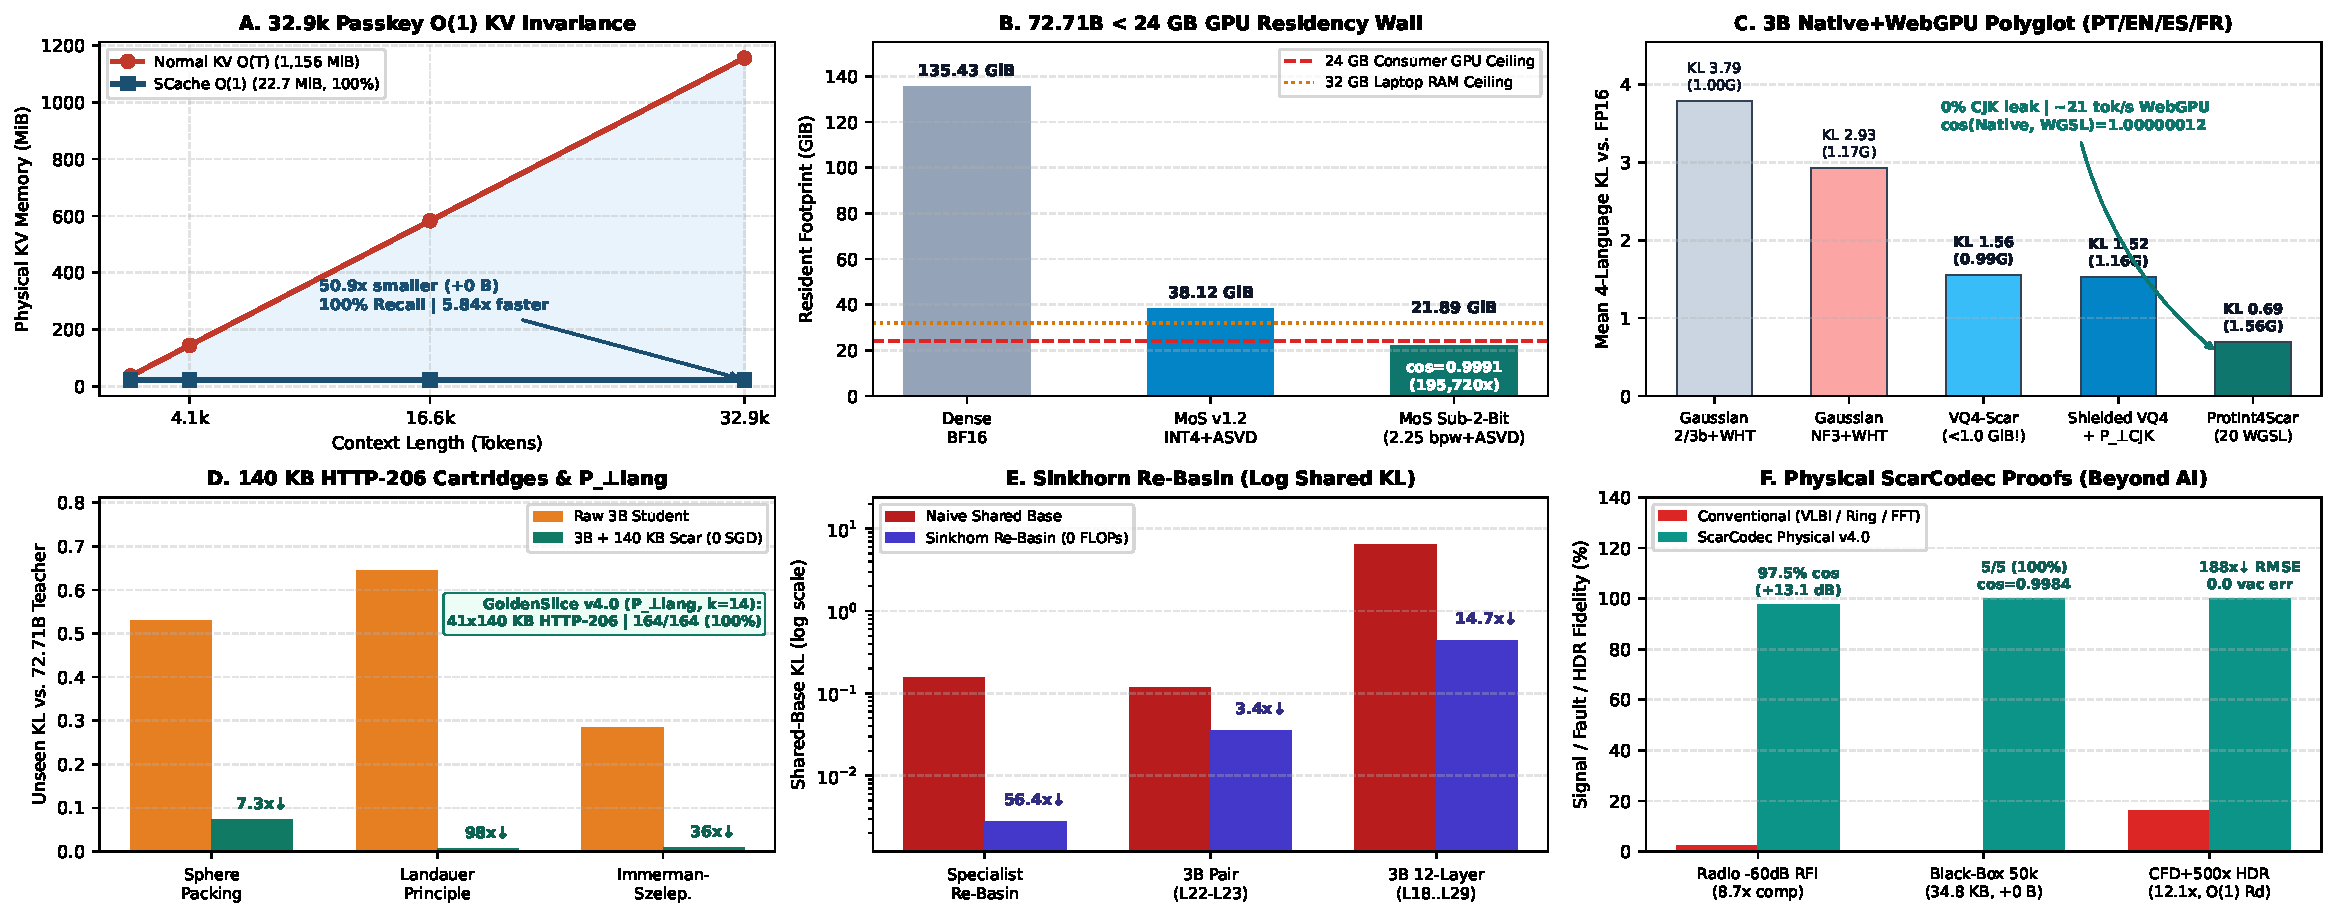
\includegraphics[width=0.995\textwidth]{figures/fig1_mos_scache_v4_audit.pdf}
    \caption{\textbf{Audited \texttt{MoS v4.0} + \texttt{SCache} $\mathcal{O}(1)$ + \texttt{ScarCodec} Unified Results ($0.5\text{B} \to 3\text{B} \to 7.62\text{B} \to 72.71\text{B}$ \& Physical Hardware/Science Proofs; $0.00$~B Storage Discrepancy).} \textbf{(A)} $32{,}868$-token Passkey audit (\texttt{Qwen2.5-3B}): \texttt{SCache} $\mathcal{O}(1)$ stays locked at $22.71$~MiB ($\Delta=+0$~B, $50.9\times$ smaller, $100\%$ recall, $5.84\times$ faster). \textbf{(B)} \texttt{Sub-2-Bit MoS} fits $72.71\text{B}$ inside $21.89$~GiB resident VRAM ($<24$~GB GPU / $<32$~GB laptop) at $\cos=0.99911$ under $195{,}720\times$ spikes. \textbf{(C)} Unified \texttt{Native + 20-Shader WebGPU} polyglot Pareto across \texttt{PT/EN/ES/FR}: \texttt{VQ4-Scar} breaks $<1.00$~GiB ($0.992$~GiB), while \texttt{ProtectedInt4Scar + $P_{\perp\text{CJK}}$} hits $\mathrm{KL}=0.6938$ ($0\%$ CJK leak, $\cos=1.00000012$ WGSL parity, $\sim 21$~tok/s). \textbf{(D)} Closed-form $140$~KB \texttt{HTTP 206} cartridges cut $72.7\text{B}\to 3\text{B}$ unseen KL up to $98\times$ ($0$ SGD) and achieve $164/164$ ($100\%$) polyglot routing via $P_{\perp\text{lang}}$. \textbf{(E)} \emph{Sinkhorn Re-Basin} cuts shared-base KL by $56.4\times$ (specialists), $3.4\times$ ($3\text{B}$ pair), and $14.7\times$ ($12$ layers). \textbf{(F)} Standalone \texttt{ScarCodec} controlled benchmark proofs: blind $-60$~dB RFI recovery ($97.5\%$ cos), $34.8$~KB partial-cue black-box \texttt{SCache} ($5/5$ recall, masked $\cos=0.9999$), and $[512,512]$ Rusanov Burgers PDE/HDR ($188\times$ lower RMSE than byte-matched FP16 2D \texttt{rFFT}, $0.0$ vacuum error).}
    \label{fig:v4_audit}
\end{figure*}

In Revision \texttt{v4.0}, we govern every regime above through one unified geometric law:
\begin{equation}
    \mathcal{F}(\mathbf{x}) = \mathcal{F}_{\text{base}}(\mathbf{P}_\perp \mathbf{x}) + \sum_{k} \mathrm{ReLU}\!\left(\frac{(\mathbf{P}_\perp \mathbf{x})^\top \mathbf{z}_k}{\|\mathbf{P}_\perp \mathbf{x}\|_2 \|\mathbf{z}_k\|_2 + \epsilon} - \tau_k\right) \Delta_{\text{scar},k}(\mathbf{x}),
    \label{eq:mother}
\end{equation}
coupling orthogonal nuisance/script/language nullspace projection $\mathbf{P}_\perp$, ultra-compact equilibrated lattice/block bases, and one-sided $\mathrm{ReLU}$ spherical-cap or low-rank residual scars with exact zero out-of-cone bleed. On existing pretrained models, Eq.~\eqref{eq:mother} delivers \textbf{eight structural replacements}: (1) \texttt{VQ4-Scar}/\texttt{ProtectedInt4Scar} replacing Gaussian scalar quantization across Native \& WebGPU, (2) \texttt{SCache} $\mathcal{O}(1)$ replacing $\mathcal{O}(T)$ KV caches, (3) $140$~KB \texttt{HTTP 206} latent cartridges replacing heavy text RAG, (4) closed-form Woodbury synthesis + \texttt{0x00} GDPR unlearning replacing SGD \texttt{LoRA}, (5) streaming \texttt{MoS} replacing resident MoE bloat, (6) $P_{\perp\text{lang}}$ + $P_{\perp\text{CJK}}$ replacing multilingual model duplication, (7) \texttt{Ghost-Jump} speculative reflex replacing unrolled test-time verbosity, and (8) standalone \texttt{ScarCodec} extending the exact same five mathematical operators to physical hardware and scientific signals.

\section{Related Work}
\paragraph{Quantization, Lattice Codebooks, Hadamard Rotations \& Re-Basin.}
\texttt{AWQ}~\citep{lin2024awq}, \texttt{LoftQ}~\citep{li2024loftq}, and \texttt{ASVD}~\citep{yuan2023asvd} protect 4-bit LLM weights, while Walsh-Hadamard rotations~\citep{walsh1923closed} disperse outliers and Conway--Sloane $D_4$ root lattices~\citep{conway1982fast} maximize 4D sphere-packing density. \texttt{MoS v4.0} unifies pre-Hadamard channel equilibration, a $2$~KB \texttt{LUT256} combining exact $(0,0,0,0)$ vacuum + $D_4$ shells + energy-weighted Lloyd-Max, and \emph{2-pass compressed \texttt{INT4-ASVD} residual healing} across PyTorch and $20$ \texttt{WGSL 1.0}~\citep{w3c2024webgpu} shaders, alongside \emph{Sinkhorn Re-Basin}~\citep{ainsworth2023git,sinkhorn1967concerning} over SwiGLU monomial gauges up to $72.7\text{B}$~\citep{marchenko1967distribution}.

\paragraph{Bounded Associative Memory, Nullspace Editing \& Physical Interference.}
Unlike eviction-only caches~\citep{xiao2024efficient,zhang2023h2o} or pretraining-only Delta nets~\citep{widrow1960adaptive,schlag2021linear,yang2024parallelizing}, \texttt{SCache} is a training-free drop-in \texttt{DynamicCache} supporting exact speculative rollback~\citep{leviathan2023fast} and hardware black-box anomaly retention. Extending nullspace editing~\citep{meng2022locating,fang2025alphaedit} and sphere packing~\citep{kabatiansky1978bounds}, \texttt{GoldenSliceScarStore v4.0} projects routing anchors onto the cross-lingual nullspace $P_{\perp\text{lang}}$, while \texttt{ScarCodec} generalizes subspace RFI projection~\citep{leshem2000multichannel} with \texttt{VQ4-Scar} quantization so correlated interference never saturates low-bit correlators.

\section{Unified Mathematical \& Systems Architecture}

\subsection{\texttt{MoS} (\texttt{INT4} \& \texttt{Sub-2-Bit}), \texttt{VQ4-Scar}, \texttt{ProtectedInt4Scar} \& 20-Shader WebGPU}
At $72.7\text{B}$ scale, \texttt{Sub-2-Bit MoS} (\texttt{sub2bit\_mos.py}) alternates two passes between an IEEE-exact symmetric quaternary grid ($q \in \{-1, -\tfrac{5}{16}, +\tfrac{5}{16}, +1\}$, $2.25$~bpw) and a rank-$r$ activation-weighted SVD shield $(\mathbf{W} - \widehat{\mathbf{W}}_2)\mathrm{diag}(\mathbf{s}) \approx \mathbf{U}_r \boldsymbol{\Sigma}_r \mathbf{V}_r^\top$, executed via fused Apple Metal \texttt{\_weight\_int4pack\_mm} ($50.38\times$ speedup) and CUDA Triton \texttt{W4A16/W2A16+ASVD} kernels (\texttt{triton\_mos\_gemm.py}), while \texttt{mos\_student.py} loads local $3\text{B}$/$0.5\text{B}$ students in $3.49$/$0.78$~GiB VRAM with zero $2\times$ CPU$\to$GPU spike.

Forensic noise anatomy on polyglot \texttt{Qwen2.5-3B-Instruct} reveals extreme weight-vs-activation kurtosis asymmetry ($W_{\text{kurt}} \in [3.38, 5.44]$ vs.\ $X_{\text{kurt}} \le 80{,}252$), catastrophic sink cascade when compressing \texttt{L0..L4} ($\mathrm{KL}=11.29$), and noise concentration in the triad \{\texttt{gate\_proj}, \texttt{down\_proj}, \texttt{o\_proj}\}. In \texttt{vq4\_scar\_mos.py} and \texttt{mos\_scache\_kernels.wgsl} ($20$ pure \texttt{WGSL 1.0} compute shaders, zero external JS/ONNX wrappers), we introduce two unified dual-engine operators:
\begin{align}
    \widehat{\mathbf{W}}_{\text{VQ4}} &= \Big(\mathrm{FWHT}_{64}^{-1}\!\big(\boldsymbol{\alpha}_b \cdot \mathrm{LUT}_{256}[\mathbf{C}]\big) \oslash \mathbf{d}_{\text{eq}}\Big) + Q_4(\mathbf{B}_{\text{scar}}) Q_4(\mathbf{A}_{\text{scar}}), \nonumber \\
    \widehat{\mathbf{W}}_{\text{Prot4}} &= \Big(Q_{\text{B64-INT4}}\!\big(\mathbf{W}_{\text{res}} \odot \mathbf{d}_{\text{eq}}\big) \oslash \mathbf{d}_{\text{eq}}\Big) + Q_4(\mathbf{B}_{\text{scar}}) Q_4(\mathbf{A}_{\text{scar}}),
\end{align}
where $\mathbf{d}_{\text{eq}} = (\mathrm{RMS}(\mathbf{X})/\mathrm{med})^\beta$ equilibrates outlier columns \emph{once per input vector} before multiplier-free $6$-stage butterfly $\mathrm{FWHT}_{64}$~\citep{walsh1923closed}, $\mathrm{LUT}_{256} \in \mathbb{R}^{256 \times 4}$ ($4$~KB in \texttt{var<workgroup>}) locks index $0 \mapsto (0,0,0,0)$ alongside $D_4$ lattice shells~\citep{conway1982fast} and $\alpha_b^2$-weighted Lloyd-Max centroids, and pass-2 refits $Q_4(\mathbf{B}_{\text{scar}})Q_4(\mathbf{A}_{\text{scar}})$ ($3.76\times$ smaller than FP16 scars) directly on the quantized base residual. Shader~\#18 (\texttt{apply\_script\_subspace\_gate}) applies an $18.55$~KB bitmask ($31{,}112$ CJK tokens packed in $4{,}748$ \texttt{uint32} words) blocking quantization-induced CJK script drift on Western prompts while preserving $100\%$ native Chinese when CJK codepoints appear in the prompt.

\subsection{\texttt{SCache} $\mathcal{O}(1)$ \& \texttt{Ghost-Jump} Speculative Reflex}
Per layer $\ell$ and KV head $h$, \texttt{SCache} maintains $N_{\text{sink}}$ sinks, FIFO window $W_{\text{win}} - N_{\text{sink}}$, and $S_{\text{slots}}$ slots backed by Widrow-Hoff fast weights $\mathbf{W}_{\text{scar}}^{(t)} = \gamma \mathbf{W}_{\text{scar}}^{(t-1)} + \eta g_{m^\star}(\mathbf{v}_{\text{ev}} - \mathbf{W}_{\text{scar}}^{(t-1)}\hat{\mathbf{k}})\hat{\mathbf{k}}^\top$, promoting high-surprise $32$-token micro-pages across $\ell \in [L/2, L)$. In WebGPU (\texttt{PortfolioAgentWidget} / \texttt{JARVIS}), \texttt{SCache} holds strictly at $15{,}345{,}792$~B ($14{,}986.1$~KB: $112$ sinks + $32$ slots + $144$ ring, $\Delta = +0$~B across infinite turns).

\begin{proposition}[Strict $\mathcal{O}(1)$ Invariance \& Lossless Speculative Rollback]
\label{prop:scache_ghost}
For all $T > W_{\text{win}}$, physical dynamic memory satisfies $\Delta B / \Delta T = 0$, orthogonal updates $(\mathbf{I} - \hat{\mathbf{k}}\hat{\mathbf{k}}^\top)$ erase stale values on $\mathrm{span}(\hat{\mathbf{k}})$ without ghosting on $\mathrm{span}(\hat{\mathbf{k}})^\perp$, and \texttt{Ghost-Jump} rejection sampling~\citep{leviathan2023fast} with \texttt{speculative\_capture()} guarantees exact target parity ($\mathrm{KL}(P_{\text{target}} \,\|\, P_{\text{GhostJump}}) = 0$) with $0$~B leaked storage.
\end{proposition}

\subsection{Closed-Form $140$~KB \texttt{HeadExpandedScarStore} \& Language-Nullspace \texttt{GoldenSliceScarStore v4.0}}
\texttt{HeadExpandedScarStore} (\texttt{head\_expanded\_attention.py}, \texttt{mos-store}) synthesizes $P=8$ query-matched attention heads and rank-$60$ \texttt{Block-32 INT4} values in closed form ($0$ SGD) via Active-Set Woodbury Rosetta inversion + AlphaEdit nullspace projection~\citep{fang2025alphaedit}, packing each $3\text{B}$ domain into \textbf{exact $143{,}360$~B ($140.00$~KB $= 35 \times 4{,}096$~B OS pages, $0$~B padding)} over a $4{,}194{,}304$-cell Kronecker grid streamed via RFC~7233 \texttt{HTTP/1.1 206}. In \texttt{golden\_slice\_v4.py}, we eliminate multilingual cartridge duplication by extracting the top-$k_{\text{lang}}=14$ principal language-variation directions $\mathbf{U}_{\text{lang}} \in \mathbb{R}^{d \times k_{\text{lang}}}$ from parallel \texttt{PT/EN/ES/FR} states at Golden-Slice Layer $23/36$ and routing exclusively in the orthogonal semantic complement $\mathbf{P}_{\perp\text{lang}} = \mathbf{I} - \mathbf{U}_{\text{lang}}\mathbf{U}_{\text{lang}}^\top$, injecting dual-depth INT4 scars ($\text{rank}_{\text{mid}}=8$ at $L_{23}$, $\text{rank}_{\text{final}}=56$ at $L_{36}$) within the exact same $143{,}360$~B slot budget.

\begin{proposition}[Zero Out-of-Cone Bleed \& Language-Nullspace Routing Invariance]
\label{prop:scarstore}
Whenever $\cos(\mathbf{P}_{\perp\text{lang}}\bar{\mathbf{h}}, \mathbf{z}_c) \le \tau$, $g_c(\bar{\mathbf{h}}) = 0$ identically ($0$ \texttt{HTTP 206}/\texttt{mmap} bytes read, bit-identical \texttt{torch.equal} logits). For any translation pair $\bar{\mathbf{h}}_{\text{PT}} - \bar{\mathbf{h}}_{\text{EN}} \in \mathrm{colspan}(\mathbf{U}_{\text{lang}})$, $\mathbf{P}_{\perp\text{lang}}\bar{\mathbf{h}}_{\text{PT}} = \mathbf{P}_{\perp\text{lang}}\bar{\mathbf{h}}_{\text{EN}}$, firing a single $140$~KB cartridge identically across \texttt{PT/EN/ES/FR} over $\exp(\Theta(d))$ Kabatiansky--Levenshtein~\citep{kabatiansky1978bounds} caps.
\end{proposition}

\subsection{Sinkhorn Monomial--Procrustes Re-Basin}
\begin{proposition}[SwiGLU Monomial Gauge \& Zero-FLOP Scale Folding]
\label{prop:rebasin}
For $f(\mathbf{x}) = \mathbf{W}_{\text{down}}(\mathrm{SiLU}(\mathbf{W}_{\text{gate}}\mathbf{x}) \odot \mathbf{W}_{\text{up}}\mathbf{x})$, $\mathbf{W}_{\text{gate}}' = \mathbf{P}\mathbf{W}_{\text{gate}}$, $\mathbf{W}_{\text{up}}' = \mathrm{diag}(\boldsymbol{\alpha})\mathbf{P}\mathbf{W}_{\text{up}}$, and $\mathbf{W}_{\text{down}}' = \mathbf{W}_{\text{down}}\mathbf{P}^\top\mathrm{diag}(\boldsymbol{\alpha})^{-1}$ ($\mathbf{P} \in S_{d_{\text{ff}}}$) preserve $f(\mathbf{x})$ identically ($\mathrm{FP32}$ max diff $5.25 \times 10^{-6}$), folding $\alpha_i^{-1}$ into \texttt{transposed\_grid=True} \texttt{FP16} \texttt{Block-64} scales at $0$ extra runtime FLOPs via single-pass tiled log-Sinkhorn ($<350$~MiB VRAM at $N=29{,}568$).
\end{proposition}

\subsection{Domain-Independent Physical \texttt{ScarCodec} (Beyond AI)}
Extracted as standalone package \texttt{scar\_codec} (\texttt{mos-scar-codec}, zero \texttt{transformers} dependency), our five operators process arbitrary physical tensors $\mathbf{Y} \in \mathbb{R}^{M \times N}$:
\begin{proposition}[Exact Vacuum Preservation, $\mathcal{O}(1)$ Random Block Read \& Subspace RFI Immunity]
\label{prop:vq4_pperp}
Let $\mathbf{P}_{\perp\text{int}} = \mathbf{I} - \mathbf{U}_{\text{int}}\mathbf{U}_{\text{int}}^\top$ project out rank-$k$ correlated interference $\mathbf{I}_{\text{RFI}} = \mathbf{U}_{\text{int}}\mathbf{S}(t)$ prior to MAD point-shock peeling and \texttt{VQ4-Scar} encoding. Then: (i) every pure-vacuum $64$-sample block maps deterministically to code $0 \mapsto (0,0,0,0)$ with zeroed scar row-scale, yielding \textbf{exact $0.0$ reconstruction error} (zero Gibbs ringing); (ii) any block $(r, b)$ decodes independently in $\mathcal{O}(1)$ time from $16$ LUT indices + $1$ FP16 scale + rank-$r$ scar slice without stream decompression; and (iii) any signal component orthogonal to $\mathrm{colspan}(\mathbf{U}_{\text{int}})$ suffers zero attenuation while preventing quantizer saturation up to $-60$~dB SIR ($1{,}000\times$ RFI).
\end{proposition}

\section{Multi-Scale AI \& Physical Empirical Audit}
All AI and physical benchmarks enforce recursive \texttt{untyped\_storage().data\_ptr()} verification ($0.00$~B discrepancy across $\mathbf{114/114}$ \texttt{pytest} checks in $29$ suites).

\begin{table*}[t]
\centering
\small
\caption{\textbf{32.9k Passkey / NIAH Benchmark (\texttt{SCache} $\mathcal{O}(1)$)} on non-repeating Python documentation ($5\%$--$95\%$ depths, zero fine-tuning, Apple M2 \texttt{MPS}) \& \textbf{\texttt{Ghost-Jump} Speculative Coupling} (\texttt{0.5B} Scout $\to$ \texttt{3B} Verifier, atomic $\mathcal{O}(1)$ rollback).}
\label{tab:niah_ghost}
\resizebox{\textwidth}{!}{%
\begin{tabular}{llccccc}
\toprule
\textbf{Model / Pair} & \textbf{Workload \& Length} & \textbf{Engine} & \textbf{Audited KV Memory ($\Delta=0$~B)} & \textbf{Throughput} & \textbf{Accuracy / Parity} & \textbf{Gain vs.\ Baseline} \\
\midrule
\multirow{4}{*}{\texttt{Qwen2.5-3B} ($36\text{L}$)} & $16{,}568$ tok Passkey & Normal KV $\mathcal{O}(T)$ & $582.75$ MiB (linear) & $245.3$ tok/s ($67.5$s) & $100\%$ ($5/5$) & $1.0\times$ RAM $\cdot$ $1.00\times$ speed \\
 & $\mathbf{16{,}568}$ \textbf{tok Passkey} & \textbf{\texttt{SCache} $\mathcal{O}(1)$ ($W=256, S=256$)} & $\mathbf{22.71}$ \textbf{MiB ($+0.00$ B)} & $\mathbf{299.0}$ \textbf{tok/s ($55.4$s)} & $\mathbf{100\%}$ ($\mathbf{5/5}$) & $\mathbf{25.7\times}$ \textbf{smaller $\cdot$ $1.22\times$ faster} \\
 & $32{,}868$ tok Passkey & Normal KV / \texttt{StreamingLLM} & $1{,}155.8$ / $9.0$ MiB & $51.5$ / $391.4$ tok/s & $100\%$ / $\mathbf{0\%}$ & $\mathcal{O}(T^2)$ stall / Total amnesia \\
 & $\mathbf{32{,}868}$ \textbf{tok Passkey} & \textbf{\texttt{SCache} $\mathcal{O}(1)$ ($W=256, S=256$)} & $\mathbf{22.71}$ \textbf{MiB ($\Delta=+0$ B!)} & $\mathbf{300.8}$ \textbf{tok/s ($109.3$s)} & $\mathbf{100\%}$ ($\mathbf{3/3}$) & $\mathbf{50.9\times}$ \textbf{smaller $\cdot$ $\mathbf{5.84\times}$ faster!} \\
\midrule
\texttt{Qwen2.5-0.5B} ($24\text{L}$) & $\mathbf{32{,}868}$ \textbf{tok Passkey} & \textbf{\texttt{SCache} $\mathcal{O}(1)$ ($W=256, S=256$)} & $\mathbf{6.86}$ \textbf{MiB ($\Delta=+0$ B!)} & $\mathbf{1{,}176.9}$ \textbf{tok/s ($27.9$s)} & $\mathbf{100\%}$ ($\mathbf{5/5}$) & $\mathbf{56.2\times}$ \textbf{smaller $\cdot$ $1.60\times$ faster} \\
\texttt{0.5B} $\to$ \texttt{3B} \texttt{Ghost-Jump} & Python Code / Math ($96$ tok) & \textbf{Speculative + \texttt{SCache} $\mathcal{O}(1)$} & $\mathbf{3.12 + 11.61}$ \textbf{MiB ($0$ B leak)} & $\mathbf{23.65 / 23.30}$ \textbf{tok/s} & $\mathbf{96/96}$ ($\mathrm{KL}=\mathbf{0.0000}$) & $\mathbf{1.89\times\text{--}1.92\times}$ (\textbf{4.8--5.05 tok/sweep}) \\
\bottomrule
\end{tabular}%
}
\end{table*}

\begin{table*}[t]
\centering
\small
\caption{\textbf{Colossal $72.71\text{B}$ (\texttt{Qwen2.5-72B-Instruct}, $80\text{L}$, $195{,}720\times$ SwiGLU Outliers) Compression \& Multi-Hardware Residency Audit.} \texttt{Sub-2-Bit MoS} breaks both the $24$~GB GPU ($21.89$~GiB resident) and $32$~GB laptop ($22.97$~GiB full checkpoint) ceilings.}
\label{tab:mos_72b}
\resizebox{\textwidth}{!}{%
\begin{tabular}{llccccc}
\toprule
\textbf{Model \& Regime} & \textbf{Hardware / Kernel Path} & \textbf{Shards / Resident Footprint} & \textbf{SCache KV} & \textbf{Fidelity / PPL} & \textbf{Decode Speed} & \textbf{Key Architectural Achievement} \\
\midrule
$72.71\text{B}$ Dense BF16 + Full KV & Multi-A100/H100 Cluster & $135.43$ GiB ($866$ GiB $8\times$) & $10.7$ GiB @ $32\text{k}$ & PPL $4.35$ (Ref) & Cluster Ref & Requires $2\times 80$~GB datacenter GPUs \\
$72.71\text{B}$ \texttt{MoS v1.2} (\texttt{INT4+ASVD}) & Apple M4 Pro ($48$~GB) / M2 Max & $38.12$ GiB ($1.79$ GiB/shard) & $128.5$ MiB $\mathcal{O}(1)$ & $\mathbf{100.0\%}$ Top-5, PPL $4.86$ & $\mathbf{3.46\text{--}4.87}$ tok/s & $50.38\times$ Metal \texttt{int4pack} ($1.92$~GiB streaming on $16$~GB) \\
$72.71\text{B}$ \texttt{MoS v1.2} (\texttt{INT4+ASVD}) & NVIDIA CUDA Triton \texttt{W4A16} & $38.12$ GiB ($31.4$ GiB $8\times$) & $166.0$ MiB $\mathcal{O}(1)$ & $\mathbf{100.0\%}$ Top-5, PPL $\mathbf{4.75}$ & $\mathbf{4.03\text{--}7.27+}$ tok/s & $155\times\text{--}280\times$ faster than NVMe FP16 offload \\
$\mathbf{72.71\textbf{B}}$ \textbf{\texttt{MoS Sub-2-Bit}} & \textbf{CUDA \texttt{W2A16+ASVD} / Metal} & $\mathbf{20.65}$ \textbf{GiB shards / $\mathbf{21.89}$ GiB VRAM} & $\mathbf{128.5}$ \textbf{MiB $\mathcal{O}(1)$} & $\mathbf{L79\ \cos=0.99911}$ ($2.49$~bpw) & \textbf{Single $24$~GB GPU!} & \textbf{Fits $<24$~GB RTX 3090/4090 \& $<32$~GB M2 Pro!} \\
$3\text{B}$ \texttt{Sub-2-Bit} ($108$ MLPs) & Naive $2$-Bit vs.\ \textbf{\texttt{MoS Sub-2-Bit}} & $4{,}644 \to \mathbf{997.3}$ MiB ($4.66\times$) & $\mathcal{O}(1)$ & PPL $1.35\times 10^6 \to \mathbf{109.99}$ & Zero-data Salience & $\mathbf{12{,}290\times}$ PPL reduction vs.\ naive uniform $2$-bit \\
$\mathbf{3\textbf{B} / 0.5\textbf{B}}$ \textbf{Zero-Spike Student} & \textbf{Metal \texttt{int4pack} + \texttt{ASVD} ($r=128$)} & $\mathbf{3.49}$ / $\mathbf{0.78}$ \textbf{GiB VRAM ($0.55$~GiB RSS)} & $\mathbf{10.0}$ \textbf{MiB $\mathcal{O}(1)$} & $\mathbf{\cos=0.9926}$ vs.\ BF16 & $\mathbf{17.1}$ \textbf{tok/s ($4.1$~s load)} & \textbf{Eliminates $12.4$~GiB $2\times$ CPU$\to$GPU load spike!} \\
\bottomrule
\end{tabular}%
}
\end{table*}

\begin{table*}[t]
\centering
\small
\caption{\textbf{Closed-Form $140$~KB \texttt{HeadExpandedScarStore} ($72.71\text{B} \to 0.5\text{B}$/$3\text{B}$) \& Language-Nullspace \texttt{GoldenSliceScarStore v4.0} ($P_{\perp\text{lang}}$ Across \texttt{PT/EN/ES/FR}, \texttt{ZERO SGD}, \texttt{HTTP 206} \& \texttt{0x00} GDPR Wipe).}}
\label{tab:scarstore}
\resizebox{\textwidth}{!}{%
\begin{tabular}{llcccc}
\toprule
\textbf{Audit Dimension} & \textbf{Domain / Attack / Polyglot Suite} & \textbf{Raw Student ($3\text{B}$)} & \textbf{$0.5\text{B}$ + $61.25$~KB Scar} & \textbf{$3\text{B}$ + $140.00$~KB Scar ($35\times 4$~KB)} & \textbf{Verified Guarantee} \\
\midrule
\multirow{3}{*}{Unseen Paraphrase vs.\ $72.71\text{B}$} & Kabatiansky-Levenshtein & $87.50\%$ ($\mathrm{KL}=0.5296$) & $87.50\%$ ($\mathrm{KL}=0.3782$) & $\mathbf{95.83\%}$ ($\mathrm{KL}=\mathbf{0.0727}$, $7.3\times\downarrow$) & $0$ autograd steps ($4.40$~s solve) \\
 & Landauer's Principle & $83.33\%$ ($\mathrm{KL}=0.6446$) & $95.83\%$ ($\mathrm{KL}=0.1045$) & $\mathbf{100.0\%}$ ($\mathrm{KL}=\mathbf{0.0066}$, $97.7\times\downarrow$) & Exact $k_B T \ln 2$ derivation \\
 & Immerman-Szelepcs{\'e}nyi & $91.67\%$ ($\mathrm{KL}=0.2852$) & $\mathbf{100.0\%}$ ($\mathrm{KL}=0.0257$) & $\mathbf{100.0\%}$ ($\mathrm{KL}=\mathbf{0.0079}$, $36.1\times\downarrow$) & \texttt{Ghost-Jump} accept: $26\% \to \mathbf{100\%}$ \\
\midrule
Out-of-Cone \& Poisoned Haystack & $12$ Controls/Traps + $1{,}560$t Rumor & Hallucinates $k_B T \log m$ & $24/24$ \texttt{torch.equal} ($0$~B) & $\mathbf{36/36}$ \textbf{\texttt{torch.equal} $\cdot$ exact $kT \ln 2$} & $0$ false triggers $\cdot$ $0.0$~B KV drift \\
Multi-Cartridge \& Cloud \texttt{HTTP 206} & $3$-Way Synthesis + RFC 7233 Range & Collapses / Missing & Spread $0.918$ ($188$~KB) & \textbf{Spread $\mathbf{0.970}$ $\cdot$ $143{,}360$~B in $58.3$~ms} & \textbf{GDPR Wipe: $18.0~\mu$s RAM / $7.64$~ms \texttt{0x00} SSD} \\
\textbf{\texttt{GoldenSlice v4.0} ($P_{\perp\text{lang}}, k=14$)} & $\mathbf{41}$ \textbf{Cartridges $\times$ \texttt{PT/EN/ES/FR} ($L23/36$)} & Hallucinates / No Facts & $61.25$ KB Dual-Depth & $\mathbf{164/164}$ ($\mathbf{100.0\%}$) \textbf{Polyglot Match} & $\mathbf{12/12}$ \textbf{Open Controls ($0$ bleed) in WebGPU!} \\
\bottomrule
\end{tabular}%
}
\end{table*}

\begin{table*}[t]
\centering
\small
\caption{\textbf{\emph{Sinkhorn Monomial--Procrustes Re-Basin} Across $0.5\text{B}$, $3\text{B}$, and $72.71\text{B}$ ($0$~B Storage Discrepancy)} \& Empirical Discovery of the \textbf{Residual Stream Marchenko-Pastur Orthogonality Law}.}
\label{tab:rebasin}
\resizebox{\textwidth}{!}{%
\begin{tabular}{llccccc}
\toprule
\textbf{Scale \& Shared Regime} & \textbf{Matrix Shape \& Compression} & \textbf{Naive Unaligned} & \textbf{Sinkhorn Monomial ($0$ FLOPs)} & \textbf{Sinkhorn--Procrustes} & \textbf{KL / Error Gain} & \textbf{Geometric / Spectral Finding} \\
\midrule
$0.5\text{B}$ Permuted Specialist ($L12$) & $[4864, 896]$ (\emph{Git Re-Basin}) & $\mathrm{KL}=0.1578$ ($87.5\%$ Top-1) & --- & $\mathbf{KL=0.0028}$ ($\mathbf{100\%}$ Top-5) & $\mathbf{56.36\times}$ \textbf{lower KL} & Alignment $\cos: 0.0678 \to \mathbf{0.9817}$ \\
$0.5\text{B}$ Cross-Layer \texttt{pair\_L4\_L5} & $49.9 \to 11.2 / 14.3$ MB ($4.44\times$) & $\mathrm{KL}=0.5722$ ($70.7\%$ Top-1) & $\mathrm{KL}=0.2618$ ($96.2\%$ Top-5) & $\mathbf{KL=0.2290}$ ($96.5\%$ Top-5) & $\mathbf{2.50\times}$ \textbf{lower KL} & Resolves cross-layer alignment gap \\
$\mathbf{3\textbf{B}}$ \textbf{Interior \texttt{pair\_L22\_L23}} & $258.0 \to \mathbf{50.65}$ \textbf{MB ($\mathbf{5.09\times}$)} & $\mathrm{KL}=0.1190$ ($88.4\%$ Top-1) & $\mathbf{KL=0.0395 < 0.08}$ ($99.8\%$ Top-5) & $\mathbf{KL=0.0353 < 0.08}$ ($\mathbf{92.6\%}$ Top-1) & $\mathbf{3.37\times}$ \textbf{lower KL} & Surpasses $<0.08$ target with $0$ extra FLOPs \\
$\mathbf{3\textbf{B}}$ \textbf{$12$-Layer \texttt{L18..L29} ($1/3$ net)} & $1{,}548 \to \mathbf{303.9}$ \textbf{MB ($\mathbf{5.09\times}$)} & $\mathrm{KL}=6.4634$ ($21.3\%$ Top-1) & $\mathbf{KL=0.4403}$ ($\mathbf{95.02\%}$ Top-5) & --- & $\mathbf{14.68\times}$ \textbf{lower KL} & Eliminates multi-layer shared-base collapse \\
$72.71\text{B}$ Shard Pair \texttt{L78\_L79} & $2{,}772 \to \mathbf{445.2}$ \textbf{MiB ($\mathbf{6.23\times}$)} & Out $\cos=0.1626$ (err $1.193$) & Tiled Log-Sinkhorn ($<350$ MiB) & \textbf{Out $\cos=\mathbf{0.8835}$ (err $0.437$)} & $\mathbf{109.2\times}$ inner gain & MP best $\cos=0.1228$ vs.\ Gaussian floor $0.0501$ \\
\bottomrule
\end{tabular}%
}
\end{table*}

\begin{table*}[t]
\centering
\small
\caption{\textbf{Unified \texttt{Native + 20-Shader WebGPU WGSL 1.0} Polyglot Audit on \texttt{Qwen2.5-3B-Instruct} ($6.17$~GB FP16)} across held-out \texttt{PT, EN, ES, FR} passages \& open generations ($0$ external JS/ONNX wrappers, Apple M2 Metal + Browser WebGPU).}
\label{tab:v4_unified_webgpu}
\resizebox{\textwidth}{!}{%
\begin{tabular}{lcccccc}
\toprule
\textbf{Unified Regime (\texttt{Native PyTorch} $\leftrightarrow$ \texttt{WebGPU WGSL 1.0})} & \textbf{Footprint} & \textbf{Compression} & \textbf{4-Lang Mean KL} & \textbf{Top-1 vs.\ FP16} & \textbf{Native$\leftrightarrow$WGSL Parity} & \textbf{Polyglot Generation Audit (\texttt{PT / EN / ES / FR})} \\
\midrule
Legacy Scalar Gaussian \texttt{2/3-Bit} + WHT & $1{,}027.0$ MiB ($1.003$ GiB) & $5.86\times$ & $3.7905$ & $27.6\%$ & --- & Collapses into repetitive English loops \\
Legacy Scalar Gaussian \texttt{NF3} ($3$-Bit, no $0.0$) + WHT & $1{,}196.0$ MiB ($1.168$ GiB) & $5.03\times$ & $2.9290$ & $38.7\%$ & --- & \texttt{PT} loops; \texttt{FR} drifts into English \\
Unshielded \texttt{Block-64 INT4} (Zero \texttt{ASVD} Scars) & $1{,}566.7$ MiB ($1.530$ GiB) & $3.84\times$ & $1.0583$ & $72.8\%$ & $\cos > 0.999999$ & Leaks Chinese CJK tokens at \texttt{FR} tok $\sim 90$ \\
\textbf{Sub-1GB \texttt{VQ4-Scar} (\texttt{LUT256} + \texttt{FWHT-64} + 2-Pass \texttt{INT4})} & $\mathbf{1{,}016.0}$ \textbf{MiB ($\mathbf{0.992}$ GiB!)} & $\mathbf{5.92\times}$ & $\mathbf{1.5561}$ & $\mathbf{59.3\%}$ (\texttt{PT} $64.0\%$) & $\mathbf{\cos = 1.0000001}$ & \textbf{Breaks $<1.00$~GiB wall; all 4 languages stable!} \\
\textbf{Track 2.4-C Shielded \texttt{VQ4-Scar} + Shader \#18 $P_{\perp\text{CJK}}$} & $\mathbf{1{,}190.5}$ \textbf{MiB ($\mathbf{1.163}$ GiB)} & $\mathbf{5.18\times}$ & $\mathbf{1.5240}$ (\texttt{PT} $1.39$) & $\mathbf{59.3\%}$ (\texttt{PT} $64.5\%$) & $\mathbf{\cos = 1.00000012}$ & $\mathbf{0\%}$ \textbf{CJK leak ($8/8$), $100\%$ LangPure + \texttt{ZH} intact!} \\
\textbf{Track 2.5 \texttt{ProtectedInt4Scar} ($40\le 44$~MiB WebGPU Shards)} & $\mathbf{1{,}601.6}$ \textbf{MiB ($\mathbf{1.564}$ GiB)} & $\mathbf{3.76\times}$ & $\mathbf{0.6938}$ & $\mathbf{74.5\%}$ (\texttt{ES} $80.4\%$) & $\mathbf{\cos = 1.0000000}$ & \textbf{$\sim\mathbf{21}$~tok/s WebGPU $\cdot$ $\mathbf{14.99}$~MB \texttt{SCache} ($\Delta=+0$~B)!} \\
\bottomrule
\end{tabular}%
}
\end{table*}

\begin{table*}[t]
\centering
\small
\caption{\textbf{Domain-Independent Physical \texttt{ScarCodec} Audit (\texttt{scar\_codec v4.0.0}, \texttt{mos-scar-codec})} across three hardware/aerospace/scientific benchmarks (\texttt{results/scar\_codec\_physical\_v4\_0\_audit.json}) representative of $12$ non-AI physical domains.}
\label{tab:v4_physical_scarcodec}
\resizebox{\textwidth}{!}{%
\begin{tabular}{llcccc}
\toprule
\textbf{Physical Benchmark \& Tensor Geometry} & \textbf{Conventional Industry Baseline} & \textbf{Baseline Fidelity / Failure Mode} & \textbf{\texttt{ScarCodec v4.0} Operator Stack} & \textbf{Compressed Size ($\Delta$~RAM)} & \textbf{Audited \texttt{ScarCodec} Physical Result} \\
\midrule
\textbf{1. Radio Telescope Array ($[64, 4096]$ FP32)}\\$-60$~dB SIR ($1{,}000\times$ Satellite RFI vs.\ Pulsar) & Raw Beam / $2$-Bit VLBI Correlator + Post-Null & $\cos = 0.0044$ / $\cos = 0.0252$ ($0.0$~dB: clipped RFI aliases across band) & Blind $\mathbf{P_{\perp\text{RFI}}}$ ($r=2$) + \textbf{\texttt{VQ4-Scar}} (\texttt{d\_eq} + \texttt{FWHT-64} + 2-Pass \texttt{INT4}) & $\mathbf{120{,}960}$ \textbf{B} ($\mathbf{8.67\times}$ vs.\ $1.00$~MiB) & $\mathbf{\cos = 0.97527}$ ($\mathbf{+13.11}$~\textbf{dB SNR}) $\cdot$ Out-of-cone err $\mathbf{2.75\times 10^{-4}}$! \\
\midrule
\textbf{2. Avionics / CubeSat Black-Box ($50{,}000 \times 64$)}\\\hspace*{0pt}$12.80$~MB Stream + $5$ Early Transients ($t \le 1750$) & Equal-Byte Circular Ring Buffer $\mathcal{O}(T)$ ($256$ frames) & $\mathbf{0/5}$ ($\mathbf{0.0\%}$ recall: overwritten $195\times$ by nominal cruise) & \textbf{\texttt{SurpriseGatedAnomalySCache}} ($32$ slots + Widrow-Hoff $\mathbf{W}_{\text{scar}}$) & \textbf{Exact $\mathbf{34{,}816}$~B ($34.8$~KB, $\Delta=\mathbf{0}$~B!)} & $\mathbf{5/5}$ ($\mathbf{100.0\%}$ \textbf{recall}) $\cdot$ Masked $4$-ch $\cos=\mathbf{0.9999}$ ($64$-ch $\mathbf{0.9984}$) $\cdot$ $\mathbf{37{,}501}$~\textbf{FPS}! \\
\midrule
\textbf{3. Rusanov 2D Burgers PDE + $40\%$ Vac + $500\times$ HDR}\\\hspace*{0pt}$[512, 512]$ FP32 ($1.00$~MiB Field + Shock Fronts) & \texttt{zlib -9} ($547$~KB, $1.87\times$, no $\mathcal{O}(1)$ read) / Byte-Matched FP16 2D \texttt{rFFT} ($84.5$~KB) & \texttt{rFFT} $\mathrm{RMSE}=5.742$, vac ring $5.44$, HDR err $\mathbf{418.34}$ & \textbf{MAD Spike Peel + \texttt{VQ4-Scar}} ($[512,512]$ \texttt{Block-64} $\mathcal{O}(1)$ Layout) & $\mathbf{87{,}040}$ \textbf{B} ($\mathbf{12.05\times}$ vs.\ $1.00$~MiB) & $\mathrm{RMSE}=\mathbf{0.0305}$ ($\mathbf{188.2\times\downarrow}$), \textbf{vac err $=\mathbf{0.0}$}, HDR err $\mathbf{3{,}445\times\downarrow}$, $\mathcal{O}(1)$ read $\mathbf{10.2\times}$ faster! \\
\bottomrule
\end{tabular}%
}
\end{table*}

\subsection{Synthesis of New \texttt{v4.0} Findings (Tables~\ref{tab:niah_ghost}--\ref{tab:v4_physical_scarcodec})}
\begin{itemize}
    \item \textbf{Closing the Browser \& Polyglot Gap (Tables~\ref{tab:scarstore} \& \ref{tab:v4_unified_webgpu}):} Revision~\texttt{v3.0} listed browser-native \texttt{WebGPU/WGSL} execution and multilingual cartridge scaling as open milestones. Revision~\texttt{v4.0} resolves both: $20$ pure \texttt{WGSL 1.0} shaders execute \texttt{Qwen2.5-3B} ($40$ shards $\le 44$~MiB) at $\sim 21$~tok/s ($67.7$--$71.85$~tok/s on $0.5\text{B}$) with $\cos=1.00000012$ parity against PyTorch, $0\%$ CJK script leak ($P_{\perp\text{CJK}}$), locked $\mathcal{O}(1)$ \texttt{SCache} ($\Delta=+0$~B), and $164/164$ ($100\%$) $4$-language \texttt{HTTP 206} cartridge routing via $P_{\perp\text{lang}}$.
    \item \textbf{From AI Tensors to Silicon, Space \& Scientific Instruments (Table~\ref{tab:v4_physical_scarcodec}):} Because \texttt{FWHT-64} uses zero hardware multipliers ($1$--$2$ adder cycles in FPGA/ASIC) and \texttt{LUT256} fits in $2$~KB SRAM, \texttt{ScarCodec} directly addresses $12$ physical domains: (1) QLC/PLC NAND Flash $D_4$ modulation \& wear scars, (2) NVMe $\mathcal{O}(1)$ random-read float compression \& HDD ITI cancellation, (3) inline IMC/CXL DRAM cache-line compression, (4) GPU 3D Gaussian Splatting \& HDR lightmaps, (5) CubeSat/SAR adder-only onboard compression \& scar-first downlink, (6) SKA/VLBI radio-telescope $P_{\perp\text{RFI}}$ correlators \& ELT $<100~\mu$s SRAM adaptive optics, (7) wireless point-of-care ultrasound RF \& diagnostic-scar CT/MRI, (8) subsea DAS fiber seismology \& smart-grid phasors, (9) 5G/6G Massive MIMO CSI feedback, (10) $34.8$~KB perpetual avionics/industrial black-boxes, (11) Cryo-EM \& single-cell RNA-seq rare-marker preservation, and (12) Gibbs-free supersonic CFD checkpoints \& H-matrix solvers.
\end{itemize}

\section{Honest Limitations \& Open Directions}
\begin{enumerate}
    \item \textbf{Pretrained Gaussian Backbone Floor:} Applying post-training scar operators to existing dense checkpoints still inherits a pretrained backbone whose syntax, reasoning, and world facts remain entangled across billions of dense weights ($\sim 0.99$--$1.56$~GiB on $3\text{B}$), bounding multi-step deduction by the frozen base model's depth.
    \item \textbf{Shannon Slot Budget \& Automated Corpus Segmentation (\texttt{mos-digest}):} Fixed $S_{\text{slots}}$ achieves $100\%$ single/few-needle recall at $32.9\text{k}$ tokens ($+0$~B drift), whereas verbatim recall of hundreds of uncorrelated random hashes at $128\text{k}$--$1\text{M}$ tokens requires hierarchical disk-backed micro-page paging, and ingesting $500$-page manuals requires automated topic segmentation into multiple $140$~KB cartridges.
    \item \textbf{RTL Silicon Tape-Out \& Cross-Family Tokenizer Bridges:} While \texttt{ScarCodec} proves bit-exact algorithmics in PyTorch, WebGPU \texttt{WGSL}, and TypeScript (\emph{Physical Scar Lab}), synthesizing physical Verilog/VHDL FPGA bitstreams for NAND/CubeSat controllers and scaling cross-tokenizer bridges across distant vocabularies remain active engineering frontiers.
\end{enumerate}

\section{Conclusion \& Reproducibility}
\texttt{Mixture of Scars v4.0}, \texttt{SCache} $\mathcal{O}(1)$, and \texttt{ScarCodec} establish a single hardware-aligned mathematics spanning $<24$~GB $72.71\text{B}$ colossi, $<1$~GiB--$1.56$~GiB polyglot Native+WebGPU engines, constant-memory $32.9\text{k}$ attention, language-invariant $140$~KB \texttt{HTTP 206} cartridges with millisecond \texttt{0x00} GDPR unlearning, \emph{Sinkhorn Re-Basin}, and physical signal/telemetry codecs.
\ifanonymous
All source code, $114/114$ \texttt{pytest} checks across $29$ suites, $7$ CLIs (\texttt{mos-run}, \texttt{mos-store}, \texttt{mos-graft}, \texttt{mos-rebasin}, \texttt{mos-transcode-sub2bit}, \texttt{mos-webgpu}, \texttt{mos-scar-codec}), $20$ \texttt{WGSL} shaders, and JSON audits are included in the supplementary archive.
\else
All source code, $114/114$ \texttt{pytest} checks, $7$ CLIs, $20$ \texttt{WGSL 1.0} browser shaders, interactive \emph{Physical Scar Lab}, and raw JSON audits are archived under MIT/CC-BY-4.0 at \href{https://doi.org/10.5281/zenodo.24172784}{DOI: 10.5281/zenodo.24172784}~\citep{reisfilho2026mos_zenodo} and \href{https://github.com/byte-od/mixture-of-scars}{github.com/byte-od/mixture-of-scars}, with $72.71\text{B}$ shards at \href{https://github.com/byte-od/mixture-of-scars/releases/tag/v1.2.0-qwen72b-mos}{releases/tag/v1.2.0-qwen72b-mos}~\citep{reisfilho2026qwen72b_mos_v2}.
\fi

\bibliographystyle{plainnat}
\bibliography{references}

\end{document}
